% DRAFT -- not for submission. Claims, references, results and authorship
% have not been reviewed (research/paper/README.md). Every number in the
% prose is a macro from ../tables/numbers.tex, generated from the result
% files by research/scripts/tables.py; tables and figures are \input from
% generated files. Do not type numbers by hand.
\documentclass[11pt]{article}
\usepackage[margin=2.5cm]{geometry}
\usepackage[T1]{fontenc}
\usepackage{lmodern}
\usepackage{microtype}
\usepackage{booktabs}
\usepackage{tabularx}
\usepackage{amsmath,amssymb}
\usepackage{tikz}
\usepackage{xcolor}
\usepackage{graphicx}
\usepackage[numbers,sort&compress]{natbib}
\usepackage[hidelinks]{hyperref}
\usepackage{enumitem}

% Generated by research/scripts/tables.py -- do not edit by hand.
\newcommand{\RetroEvents}{27}
\newcommand{\RetroPairs}{167}
\newcommand{\RetroInScope}{103}
\newcommand{\RetroOutScope}{62}
\newcommand{\RetroDeterminable}{165}
\newcommand{\EventsAtRisk}{27}
\newcommand{\FCa}{35}
\newcommand{\FCaEvents}{10}
\newcommand{\FCc}{0}
\newcommand{\FCcUpper}{0.035}
\newcommand{\FCcEventUpper}{0.105}
\newcommand{\FCbinary}{26}
\newcommand{\FCbinaryEvents}{8}
\newcommand{\SignAp}{0.0010}
\newcommand{\SignBinaryp}{0.0039}
\newcommand{\UnresA}{0}
\newcommand{\UnresB}{97}
\newcommand{\UnresV}{87}
\newcommand{\UnresC}{64}
\newcommand{\ResA}{128}
\newcommand{\ResB}{68}
\newcommand{\ResV}{78}
\newcommand{\ResC}{96}
\newcommand{\FPa}{2}
\newcommand{\FPc}{1}
\newcommand{\ComplChanged}{7}
\newcommand{\IdAblMiss}{17}
\newcommand{\NameIdMiss}{35}
\newcommand{\NoCurAffectedDrop}{16}
\newcommand{\NoCurUnresRise}{20}
\newcommand{\PairsPerEvent}{6.19}
\newcommand{\MatrixCases}{6,195}
\newcommand{\RandCases}{100,000}
\newcommand{\InvCases}{12,000}
\newcommand{\InvViolations}{0}
\newcommand{\MutCaught}{23}
\newcommand{\MutTotal}{23}
\newcommand{\MutByInv}{14}
\newcommand{\MutNotReinjected}{3}
\newcommand{\MutKnown}{26}
\newcommand{\FCaBoot}{[0.170, 0.520]}
\newcommand{\BootResamples}{10,000}
\newcommand{\BootSeed}{20261031}
\newcommand{\NegC}{25}
\newcommand{\NegCEvents}{13}
\newcommand{\NegCInScope}{0}
\newcommand{\NegCOther}{142}
\newcommand{\IdCurated}{29}
\newcommand{\IdSelf}{138}
\newcommand{\IdHeuristic}{0}
\newcommand{\FaultMis}{29}
\newcommand{\FaultMisMiss}{18}
\newcommand{\FaultMisNoAssoc}{11}
\newcommand{\FaultMisInScope}{18}
\newcommand{\FaultCol}{16}
\newcommand{\FaultColChanged}{0}
\newcommand{\FaultColFP}{0}
\newcommand{\LabAgreeAB}{148}
\newcommand{\LabKappaAB}{0.80}
\newcommand{\LabKappaABci}{[0.62, 0.95]}
\newcommand{\LabAdjudicated}{19}
\newcommand{\LabAgreeAPLone}{142}
\newcommand{\LabKappaAPLone}{0.72}
\newcommand{\LabKappaAPLoneci}{[0.55, 0.90]}
\newcommand{\LabDisagreeAPLone}{25}
\newcommand{\LabInAP}{91}
\newcommand{\LabUndAP}{22}
\newcommand{\LabDecidedToUnd}{22}
\newcommand{\LabAtRiskAP}{24}
\newcommand{\LabFCcA}{0}
\newcommand{\LabFCcEvA}{0}
\newcommand{\LabFCaA}{30}
\newcommand{\LabFCaEvA}{9}
\newcommand{\LabFCbinA}{23}
\newcommand{\LabFCcB}{0}
\newcommand{\LabFCcEvB}{0}
\newcommand{\LabFCaB}{30}
\newcommand{\LabFCaEvB}{9}
\newcommand{\LabFCbinB}{26}
\newcommand{\LabFCcAP}{0}
\newcommand{\LabFCcEvAP}{0}
\newcommand{\LabFCaAP}{30}
\newcommand{\LabFCaEvAP}{9}
\newcommand{\LabFCbinAP}{23}
\newcommand{\LabFCcBoundC}{0}
\newcommand{\LabFCcEvBoundC}{0}
\newcommand{\LabFCaBoundC}{35}
\newcommand{\LabFCaEvBoundC}{10}
\newcommand{\LabFCbinBoundC}{26}
\newcommand{\LabFCcBoundA}{0}
\newcommand{\LabFCcEvBoundA}{0}
\newcommand{\LabFCaBoundA}{30}
\newcommand{\LabFCaEvBoundA}{9}
\newcommand{\LabFCbinBoundA}{23}


\newcommand{\code}[1]{\texttt{#1}}
% A citation whose metadata has not been verified against a primary source
% (LITERATURE_PROTOCOL.md). Renders a dagger so it cannot pass unnoticed.
\newcommand{\citeUNV}[1]{\cite{#1}$^{\dagger}$}
\newcommand{\draftnote}[1]{\textcolor{red!70!black}{[\textbf{Draft:} #1]}}

\title{Evidence-Aware Dependency Risk Analysis:\\
A Conservative Approach to Upstream Change Applicability\\[0.5em]
\large\textcolor{red!70!black}{DRAFT --- claims, references and authorship under review}}
\author{\draftnote{authors and affiliations to be confirmed}\\ Ikarus AI Labs}
\date{Draft of 31 October 2026}

\begin{document}
\maketitle

\begin{abstract}
Software teams, and increasingly AI coding agents, decide whether an upstream
change --- a relicensing, an end of life, a registry move, a deprecation, a
compromised release --- applies to the dependencies they use. Tools answer
this from upstream records, and a common reading treats a dependency that the
record does not list as unaffected. We study how applicability can be decided
without reading incomplete, ambiguous or insufficient evidence as proof that a
dependency is unaffected. We describe an evidence-aware applicability model,
implemented in the open-source tool OpenPulse, that represents dependency
identity and how it was established, typed event scope, whether that scope was
declared complete and on what basis, evidence freshness, and an explicit
unresolved outcome that is never converted into a clearance. We state eight
decision invariants and check them as properties on \InvCases{} generated
cases with \InvViolations{} violations; of \MutTotal{} known defects and
disabled safety rules re-injected into the engine, the checks catch
\MutCaught{}. On a frozen retrospective set of
\RetroEvents{} real upstream events and \RetroPairs{} dependency references,
labelled by the developer, a naive reading of the same records cleared
\FCa{} of \RetroInScope{} in-scope references, OpenPulse cleared
\FCc{}, and the same engine read as a binary tool cleared \FCbinary{}: most of
the difference comes from keeping the unresolved outcome. The cost is
\UnresC{} unresolved outcomes. The labels are not independent and the events
were purposively selected, so these are observations on this sample, not
estimates of real-world error rates. All code, data, results and the scripts
that regenerate every table are open.
\end{abstract}

\noindent\textbf{Keywords:} software supply chain; dependency management;
software composition analysis; applicability; three-valued decisions;
reproducibility; AI coding agents.

% ---------------------------------------------------------------------------
\section{Introduction}

A team that runs \code{docker.io/bitnami/redis:7.2}, \code{node-ipc@10.1.1} or
\code{github.com/docker/docker} learns of upstream changes from announcements,
advisories and lifecycle catalogues. Each such record names what changed. The
question a team, a CI gate or an AI coding agent must answer is narrower: does
\emph{this} reference fall inside what changed?

The question is easy to answer wrongly in one direction. If the record lists
affected objects and the reference is not on the list, it is tempting to
conclude the reference is unaffected. That conclusion is only as good as three
premises that the record rarely states: that the list is complete, that the
reference was matched to the right object, and that the record is current. A
container image may be the same software under another name; a package of the
same name may be a different project in another ecosystem; a list of
``affected images'' may be a set of examples. When any premise fails, the
reader issues a \emph{false clear}: an in-scope dependency reported as
unaffected.

This paper asks:
\begin{quote}
\emph{How can dependency-risk analysis determine whether an upstream change
applies to a dependency without incorrectly interpreting incomplete,
ambiguous or insufficient evidence as proof that the dependency is
unaffected?}
\end{quote}

\paragraph{Contributions.} We distinguish the kind of evidence behind each.
\begin{enumerate}[nosep]
  \item \emph{Design.} An applicability model that makes identity, scope,
  completeness, freshness and an unresolved outcome explicit, with a negative
  admitted only under stated conditions (Section~\ref{sec:model}).
  \item \emph{Implementation and tests.} The model in OpenPulse, with eight
  decision invariants checked as properties on generated cases and a defect
  re-injection campaign that shows the checks detect the failures they target
  (Section~\ref{sec:impl}).
  \item \emph{Retrospective observation.} A comparison with a naive reading,
  conservative baselines and ablations on a frozen, developer-labelled set of
  real events (Sections~\ref{sec:method}--\ref{sec:results}), which shows
  where the reduction in false clears comes from and what it costs.
  \item \emph{Open artefact.} Code, data, labelling guide, and one command
  that regenerates and checks every table in this paper
  (Section~\ref{sec:availability}).
\end{enumerate}
We do not claim effectiveness beyond the studied sample, independent
validation, or any effect on AI coding agents; Section~\ref{sec:limits} lists
what is not shown.

% ---------------------------------------------------------------------------
\section{Background and related work}
\label{sec:related}

\draftnote{Positioning must be completed under LITERATURE\_PROTOCOL.md; in
particular SPDX~3.0 relationship completeness and CycloneDX compositions must
be read from their specifications before any novelty statement is made.}

\paragraph{Vulnerability applicability.} Software composition analysis (SCA)
maps dependencies to known vulnerabilities. Metadata matching over-reports;
code-centric approaches decide whether vulnerable code is reachable
\cite{ponta2018beyond,ponta2020detection}, and counting only deployed,
fixable dependencies changes the picture substantially
\cite{pashchenko2018vulnerable}. SCA tools disagree with one another on the
same project \cite{imtiaz2021comparative}, and the databases they read contain
errors in affected products and versions \cite{anwar2022cleaning}. Our setting
differs in the events considered --- lifecycle, licence, distribution and
ownership changes rather than vulnerabilities --- but shares the question of
when a negative may be issued.

\paragraph{Exchange formats.} OSV \cite{osvschema} and the GitHub Advisory
Database \cite{ghsa} describe affected packages and version ranges. VEX
statements, including OpenVEX \cite{openvex} and the CISA minimum requirements
\cite{cisa2023vex}, give a product status of affected, not affected, fixed or
under investigation; CSAF carries similar statements \citeUNV{oasis2022csaf}.
SBOM standards \cite{spdx,ecma424} describe what a product contains. These
formats carry \emph{statements}; the question this paper studies is how a
consumer should \emph{decide} from them when an object is not mentioned.
\draftnote{Compare with SPDX~3.0 \code{completeness} on relationships and
CycloneDX \code{compositions.aggregate}; both may express completeness of a
listing and must be discussed.}

\paragraph{Upstream lifecycle and ownership change.} Deprecation signals are
often missing or unclear \cite{cogo2022deprecation}, developers have no
systematic way to learn that a dependency was abandoned
\cite{miller2023winging}, and repository transfers and renames leave
redirects that can be hijacked \cite{github2026transfer,goldman2023repojacking}.
Supply-chain attack taxonomies include account and project takeover
\cite{ohm2020backstabber,ladisa2023sok,zimmermann2019small}. Container images
add their own identity questions: namespaces, mirrors and moving tags
\cite{shu2017dockerhub,zerouali2019outdated}.

\paragraph{Incomplete information.} Treating absence from a list as falsity
is the closed-world assumption \citeUNV{reiter1978closed}; database research
has long distinguished it from reasoning under incomplete information and
asked when a query answer can be known to be complete
\citeUNV{razniewski2011completeness}. Three-valued logics give the unknown
value its own place \citeUNV{kleene1952introduction}. Our unresolved outcome
plays that role for applicability decisions.

\paragraph{AI coding agents.} Code-generating models suggest packages that do
not exist \cite{spracklen2025package,krishna2025phantoms} and insecure code
\cite{pearce2022asleep}, and tool outputs are a channel for indirect prompt
injection \cite{greshake2023indirect,debenedetti2024agentdojo}. These motivate
giving agents structured, evidence-carrying answers in which ``unknown'' is
distinguishable from ``safe''; they do not show that doing so changes agent
behaviour, which we do not test.

% ---------------------------------------------------------------------------
\section{Research questions and hypotheses}

We evaluate three hypotheses, as hypotheses.
\begin{description}[nosep,leftmargin=1.2em]
  \item[H1] An evidence-aware applicability model makes fewer false-clear
  decisions than a specified naive reading of the same upstream records.
  \item[H2] Representing completeness, identity, scope and unresolved outcomes
  explicitly makes the causes of decision errors observable and reproducible.
  \item[H3] The approach has costs --- unresolved outcomes, identity gaps,
  review effort --- that must be measured rather than hidden.
\end{description}
H1 is an effectiveness claim; we can observe it on our sample but not
establish it in general (Section~\ref{sec:threats}). H2 is a property of the
artefact and is tested directly. H3 is measured in part: unresolved outcomes
and identity gaps are measured, review effort is not.

% ---------------------------------------------------------------------------
\section{The evidence-aware applicability model}
\label{sec:model}

\paragraph{Pairs, events and references.} A \emph{reference} $d$ is a
container reference or an (ecosystem, name, version) package. An
\emph{event} $e$ is a recorded upstream change to a project $p_e$, with
evidence items that carry a source, an authority tier, an acquisition time and
a relation (supports or contradicts). The model decides each pair $(d,e)$.

\paragraph{Identity.} $d$ resolves to a project together with \emph{how} it was
resolved: a curated explicit alias or catalogue mapping (\textsc{Verified}), a
heuristic rule (\textsc{Review-Required}), or itself (unresolved). Only a
curated, \textsc{Verified} mapping to another project is evidence that $d$ is
\emph{not} $p_e$. An unresolved or heuristic identity is never evidence of
another project, whatever the name looks like: a mirror, fork or rename can be
called anything.

\paragraph{Scope.} An event's scope is a set of typed elements --- artefact
(registry, namespace, name, with a tag, a tag predicate or a digest), release
line, package, registry --- or, if none is given, the project. An element is
\emph{exact} (everything it denotes is affected) or an \emph{envelope}
(it bounds the affected set without asserting membership). Objects an
announcement names ``for example'' are examples: they can establish membership
but never bound the scope. Each element test returns member, excluded,
undetermined, project tie or no association; every element is evaluated, and
one undetermined element withholds a clearance.

\paragraph{Completeness and admission of negatives.} A scope may be
\emph{declared complete}, and a declaration must record its basis. A
\textsc{NotAffected} verdict for $(d,e)$ is admitted only if (i) every element
of $e$'s scope decisively excludes $d$ or has no association with it, (ii) the
scope is declared complete with a recorded basis, (iii) the event is current
--- not withdrawn, superseded or contested --- and (iv) its newest evidence is
within a freshness bound (90 days by default). Otherwise the pair is
\emph{unresolved} (\textsc{Related}).

\paragraph{Outcomes and aggregation.} Per pair, the model returns one of seven
relationships, which summarise to four outcomes: \emph{affected}
(artefact, version or package membership), \emph{unresolved} (\textsc{Related},
or a project tie without established membership), \emph{cleared}
(\textsc{NotAffected}) and \emph{no association}. Across events, affected
dominates unresolved, which dominates cleared: a clearance from one event
never headlines over an unresolved association from another. Every verdict
carries a closed-vocabulary statement of what it does \emph{not} assert:
scope membership is not a finding that a dependency is broken or unsafe, and a
clearance covers only the cited event's direct scope.

\paragraph{What a clearance rests on.} A negative is sound only under premises
the model states rather than verifies (Table~\ref{tab:premises}).

\begin{table}[t]
\centering\small
\caption{Which conditions a \textsc{NotAffected} verdict verifies and which it
assumes.}
\label{tab:premises}
\begin{tabularx}{\linewidth}{lX}
\toprule
Question & Status \\
\midrule
Was a relevant event discovered? & Assumed. A verdict covers only the events supplied. \\
Was the event represented accurately, including its completeness declaration? & Assumed (trusted curation). \\
Was the reference's identity resolved correctly? & Partly checked: unresolved and heuristic identities can never exclude; a wrong curated mapping is not detected. \\
Was the scope evaluated correctly? & Checked against the specification (Section~\ref{sec:impl}). \\
Was the result communicated correctly? & Checked for the evidence contract and the agent interface. \\
\bottomrule
\end{tabularx}
\end{table}

% ---------------------------------------------------------------------------
\section{OpenPulse: design and implementation}
\label{sec:impl}

OpenPulse is a Python command-line tool and library (Apache-2.0). It reads
watchlists, SBOMs, manifests, lockfiles and image lists, evaluates them against
curated and collected events, and reports verdicts as text, JSON evidence
contracts (with a published JSON Schema), SARIF, and through a read-only Model
Context Protocol (MCP) server for coding agents. The decision engine is
\code{core/risk/match.py} and \code{core/risk/check.py}.

\paragraph{Decision invariants.} We state eight properties that no verdict may
violate (Table~\ref{tab:invariants}) and check them on the production engine's
outputs over seeded generated cases --- dependencies and one to three events
with random typed scopes, examples, completeness, basis and admissibility,
including heuristic identity mappings. The checks are stated on outputs, not on
the specification, so they also cover inputs the specification oracle does not
model.

\begin{table}[t]
\centering\small
\caption{Decision invariants, checked as properties (\code{conformance/invariants.py}).}
\label{tab:invariants}
\begin{tabularx}{\linewidth}{lX}
\toprule
I1 & An unresolved identity never yields \textsc{NotAffected} or no association under an identity-dependent scope. \\
I2 & \textsc{NotAffected} requires a complete scope with a recorded basis from a current, fresh, uncontested event. \\
I3 & As I1, for heuristic or unreviewed identity mappings. \\
I4 & An unresolved per-event verdict keeps the summary unresolved, and every machine-readable reading says it is not a clearance. \\
I5 & The evidence contract validates and states the engine's relationship; agent answers agree with the engine. \\
I6 & Look-alike elements placed first in an event never remove an affected verdict. \\
I7 & Every \textsc{NotAffected} agrees with the independent specification oracle. \\
I8 & Every verdict names its events, rules and evidence; agent answers carry the cause behind every verdict. \\
\bottomrule
\end{tabularx}
\end{table}

\paragraph{Specification oracle.} A separate implementation of the decision
procedure, written from the specification and importing nothing from the
engine, is compared with it on an exhaustive grid of \MatrixCases{} cases and
\RandCases{} randomised cases (Table~\ref{tab:conformance}).

\paragraph{Defect re-injection.} Each of \MutTotal{} known defects or
disabled safety rules is re-introduced into the running engine by a
one-function patch. The oracle
grid, the randomised differential, the invariants, a version differential and
the regression tests are run against each mutant. \MutCaught{} of
\MutTotal{} are caught; \MutByInv{} by the invariants. One defect, in which a
heuristic mapping to another project dropped an association, is invisible to
the oracle (which has no untrusted identity) and caught only by the invariants
and its regression test. It was known and open in the released version and
is fixed in the version evaluated here; no pair of the case set changes.

% Generated by research/scripts/tables.py -- do not edit by hand.
\begin{table}[t]
\centering\small
\caption{Conformance of the implementation to the specification}
\label{tab:conformance}
\resizebox{\linewidth}{!}{%
\begin{tabular}{lrr}
\toprule
check & cases & result \\
\midrule
oracle matrix (exhaustive grid) & 6195 & conform: 6123, label: both unresolved: 72 \\
randomised differential (seed 7) & 100000 & conform: 100000 \\
decision invariants I1-I8 (seeds 11, 12, 13) & 12000 & violations: 0; checks per invariant I1 2481, I2 1393, I3 1112, I4 7235, I5 12928, I6 1351, I7 1025, I8 8480 \\
defect re-injection (mutants) & 23 & caught 23; by invariants 14; not re-injected D2, D5, D6 \\
\bottomrule
\end{tabular}}
\end{table}


These are internal checks by the team that built the engine, on inputs drawn
from a finite generator vocabulary. They are evidence of conformance to the
specification, not formal verification, and not evidence that the
specification matches the world.

% ---------------------------------------------------------------------------
\section{Experimental methodology}
\label{sec:method}

\paragraph{Case set.} The retrospective set contains \RetroEvents{} upstream
events (compromised releases, deprecations, distribution changes, ends of
life, licence changes, repository relocations), each with a fixture whose
every field cites an archived primary source, and \RetroPairs{} references
found in public repositories at a commit: \RetroInScope{} in scope,
\RetroOutScope{} out of scope (look-alike names in other namespaces,
same-named packages of other projects, versions just outside a boundary, new
canonical locations) and two undeterminable. The set was frozen and
hash-pinned before any policy ran. Table~\ref{tab:retro_composition} gives its
composition.

% Generated by research/scripts/tables.py -- do not edit by hand.
\begin{table}[t]
\centering\small
\caption{Composition of openpulse-retro-2026-11 v1 (labels are the developer's, L1; none is independent)}
\label{tab:retro_composition}
\resizebox{\linewidth}{!}{%
\begin{tabular}{lrrrrrrrr}
\toprule
event class & events & pairs & in scope & out of scope & undeterminable & identity curated & identity self & identity heuristic \\
\midrule
compromised & 5 & 31 & 16 & 15 & 0 & 0 & 31 & 0 \\
deprecation & 6 & 37 & 25 & 12 & 0 & 0 & 37 & 0 \\
distribution & 6 & 39 & 24 & 15 & 0 & 0 & 39 & 0 \\
eol & 3 & 19 & 12 & 5 & 2 & 11 & 8 & 0 \\
licence & 4 & 23 & 14 & 9 & 0 & 18 & 5 & 0 \\
relocation & 3 & 18 & 12 & 6 & 0 & 0 & 18 & 0 \\
total & 27 & 167 & 103 & 62 & 2 & 29 & 138 & 0 \\
\bottomrule
\end{tabular}}
\end{table}


\paragraph{Labels.} Labels were assigned by the OpenPulse developer by written
per-event rules before any policy ran. They are not independent. Two outside
labelling rounds of a 25\% sample exist; the first followed an undocumented
process, and the second was prepared with a large language model. The study
reports both only as a pilot, not as inter-rater reliability. \draftnote{Independent
labels by two annotators with adjudication (LABELING\_GUIDE.md) would replace
this paragraph.}

\paragraph{Policies.} All policies receive the same events, replayed as known
at each event's knowledge cut, and the same reference.
\textbf{A (naive)} reads the affected list literally: listed is affected,
unlisted is cleared; identity by name, versions by release-line prefix,
references canonicalised by the oracle's parser. \textbf{B (conservative)} is
A with unlisted read as unresolved. \textbf{V (strong conservative)} is
OpenPulse's model read with each ecosystem's own version comparator.
\textbf{C} is OpenPulse. \textbf{Registered ablations} of C assume every scope
complete, drop the freshness bound, or read an unresolved identity as
unrelated. \textbf{Post-hoc ablations}, defined after the registered results
were known and therefore exploratory, read C's verdicts as binary (anything
not affected is cleared), remove curated identity, or do both with name-based
identity. An OSV/OpenVEX re-encoding baseline exists but no event of this set
has been encoded, so it is not reported.

\paragraph{Metrics.} Every rate is reported as $k/n$ with its denominator
named. The false-clear rate is false clears over in-scope pairs; the
false-positive rate is affected outcomes over out-of-scope pairs; resolution is
correct decisive outcomes over determinable pairs; the unresolved rate is over
all pairs. Pairs of one event share its evidence (\PairsPerEvent{} pairs per
event on average), so we report exact intervals that assume independence next
to event-clustered bootstrap intervals, and count false clears per event.

% ---------------------------------------------------------------------------
\section{Results}
\label{sec:results}

All numbers in this section are retrospective observations on the
developer-labelled set.

% Generated by research/scripts/tables.py -- do not edit by hand.
\begin{table}[t]
\centering\small
\caption{Decision outcomes on openpulse-retro-2026-11 by policy}
\label{tab:retro_outcomes}
\resizebox{\linewidth}{!}{%
\begin{tabular}{lrrrrrrrr}
\toprule
policy & pairs & false clears / in scope & 95\% CI (exact) & events with a false clear & false positives / out of scope & silent misses / in scope & unresolved / all & resolved / determinable [event bootstrap 95\%] \\
\midrule
A naive (listed or cleared) & 167 & 35/103 & [0.249, 0.440] & 10/27 & 2/62 & 0/103 & 0/167 & 128/165 [0.658, 0.883] \\
B conservative (listed or abstain) & 167 & 0/103 & [0.000, 0.035] & 0/27 & 2/62 & 0/103 & 97/167 & 68/165 [0.304, 0.512] \\
R OSV/OpenVEX encoding & 167 & n/a & n/a & n/a & n/a & n/a & n/a & n/a \\
V strong conservative & 167 & 0/103 & [0.000, 0.035] & 0/27 & 1/62 & 0/103 & 87/167 & 78/165 [0.333, 0.607] \\
C OpenPulse & 167 & 0/103 & [0.000, 0.035] & 0/27 & 1/62 & 0/103 & 64/167 & 96/165 [0.440, 0.714] \\
C, completeness assumed & 167 & 0/103 & [0.000, 0.035] & 0/27 & 1/62 & 0/103 & 57/167 & 103/165 [0.474, 0.764] \\
C, no freshness bound & 167 & 0/103 & [0.000, 0.035] & 0/27 & 1/62 & 0/103 & 64/167 & 96/165 [0.440, 0.714] \\
C, both assumed & 167 & 0/103 & [0.000, 0.035] & 0/27 & 1/62 & 0/103 & 57/167 & 103/165 [0.474, 0.764] \\
C, unresolved identity = unrelated & 167 & 0/103 & [0.000, 0.035] & 0/27 & 1/62 & 17/103 & 21/167 & 96/165 [0.440, 0.714] \\
C read as binary (post hoc) & 167 & 26/103 & [0.172, 0.348] & 8/27 & 1/62 & 0/103 & 0/167 & 138/165 [0.734, 0.928] \\
C without curated identity (post hoc) & 167 & 0/103 & [0.000, 0.035] & 0/27 & 1/62 & 0/103 & 84/167 & 77/165 [0.312, 0.618] \\
C with name identity only (post hoc) & 167 & 0/103 & [0.000, 0.035] & 0/27 & 1/62 & 35/103 & 12/167 & 77/165 [0.312, 0.618] \\
\bottomrule
\end{tabular}}
\end{table}


\begin{figure}[t]
\centering
\resizebox{\linewidth}{!}{% Generated by research/scripts/tables.py -- do not edit by hand.
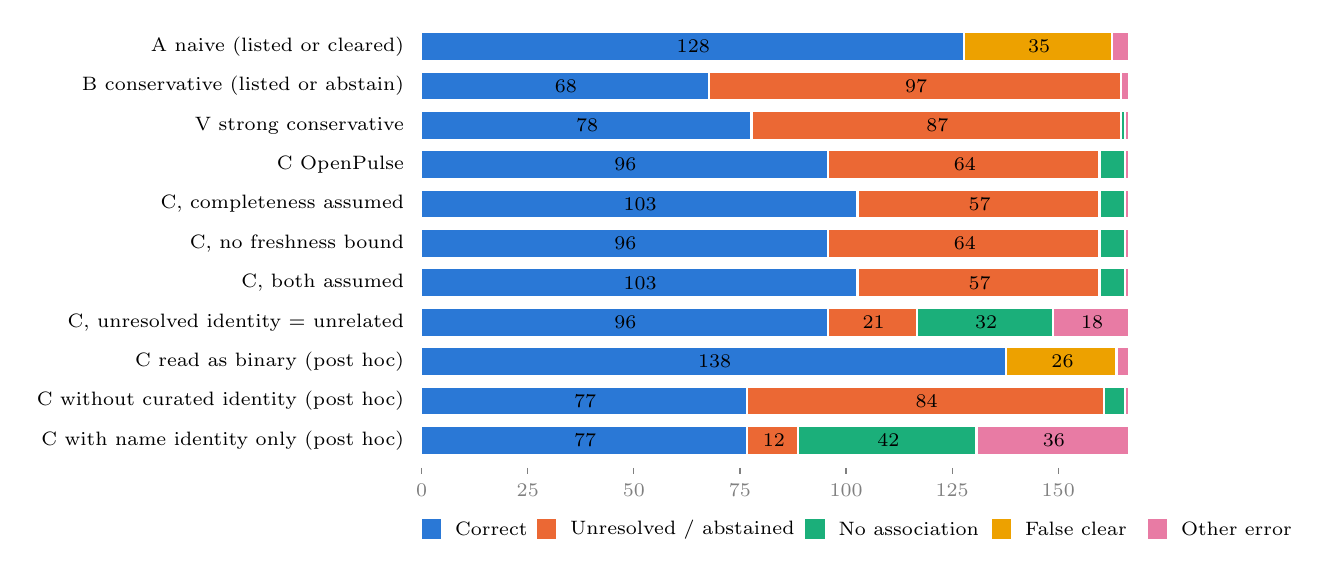
\begin{tikzpicture}[font=\scriptsize]
\definecolor{opcorrect}{HTML}{2A78D6}
\definecolor{opunresolved}{HTML}{EB6834}
\definecolor{opnoassociation}{HTML}{1BAF7A}
\definecolor{opfalseclear}{HTML}{EDA100}
\definecolor{opothererror}{HTML}{E87BA4}
\node[anchor=east] at (-0.1,-0.00) {A naive (listed or cleared)};
\fill[opcorrect] (0.000,-0.17) rectangle (6.868,0.17);
\node at (3.449,-0.00) {128};
\fill[opfalseclear] (6.898,-0.17) rectangle (8.754,0.17);
\node at (7.841,-0.00) {35};
\fill[opothererror] (8.784,-0.17) rectangle (8.970,0.17);
\node[anchor=east] at (-0.1,-0.50) {B conservative (listed or abstain)};
\fill[opcorrect] (0.000,-0.67) rectangle (3.635,-0.33);
\node at (1.832,-0.50) {68};
\fill[opunresolved] (3.665,-0.67) rectangle (8.862,-0.33);
\node at (6.278,-0.50) {97};
\fill[opothererror] (8.892,-0.67) rectangle (8.970,-0.33);
\node[anchor=east] at (-0.1,-1.00) {V strong conservative};
\fill[opcorrect] (0.000,-1.17) rectangle (4.174,-0.83);
\node at (2.102,-1.00) {78};
\fill[opunresolved] (4.204,-1.17) rectangle (8.862,-0.83);
\node at (6.548,-1.00) {87};
\fill[opnoassociation] (8.892,-1.17) rectangle (8.916,-0.83);
\fill[opothererror] (8.946,-1.17) rectangle (8.970,-0.83);
\node[anchor=east] at (-0.1,-1.50) {C OpenPulse};
\fill[opcorrect] (0.000,-1.67) rectangle (5.144,-1.33);
\node at (2.587,-1.50) {96};
\fill[opunresolved] (5.174,-1.67) rectangle (8.593,-1.33);
\node at (6.898,-1.50) {64};
\fill[opnoassociation] (8.623,-1.67) rectangle (8.916,-1.33);
\fill[opothererror] (8.946,-1.67) rectangle (8.970,-1.33);
\node[anchor=east] at (-0.1,-2.00) {C, completeness assumed};
\fill[opcorrect] (0.000,-2.17) rectangle (5.521,-1.83);
\node at (2.775,-2.00) {103};
\fill[opunresolved] (5.551,-2.17) rectangle (8.593,-1.83);
\node at (7.087,-2.00) {57};
\fill[opnoassociation] (8.623,-2.17) rectangle (8.916,-1.83);
\fill[opothererror] (8.946,-2.17) rectangle (8.970,-1.83);
\node[anchor=east] at (-0.1,-2.50) {C, no freshness bound};
\fill[opcorrect] (0.000,-2.67) rectangle (5.144,-2.33);
\node at (2.587,-2.50) {96};
\fill[opunresolved] (5.174,-2.67) rectangle (8.593,-2.33);
\node at (6.898,-2.50) {64};
\fill[opnoassociation] (8.623,-2.67) rectangle (8.916,-2.33);
\fill[opothererror] (8.946,-2.67) rectangle (8.970,-2.33);
\node[anchor=east] at (-0.1,-3.00) {C, both assumed};
\fill[opcorrect] (0.000,-3.17) rectangle (5.521,-2.83);
\node at (2.775,-3.00) {103};
\fill[opunresolved] (5.551,-3.17) rectangle (8.593,-2.83);
\node at (7.087,-3.00) {57};
\fill[opnoassociation] (8.623,-3.17) rectangle (8.916,-2.83);
\fill[opothererror] (8.946,-3.17) rectangle (8.970,-2.83);
\node[anchor=east] at (-0.1,-3.50) {C, unresolved identity = unrelated};
\fill[opcorrect] (0.000,-3.67) rectangle (5.144,-3.33);
\node at (2.587,-3.50) {96};
\fill[opunresolved] (5.174,-3.67) rectangle (6.275,-3.33);
\node at (5.740,-3.50) {21};
\fill[opnoassociation] (6.305,-3.67) rectangle (8.000,-3.33);
\node at (7.168,-3.50) {32};
\fill[opothererror] (8.030,-3.67) rectangle (8.970,-3.33);
\node at (8.515,-3.50) {18};
\node[anchor=east] at (-0.1,-4.00) {C read as binary (post hoc)};
\fill[opcorrect] (0.000,-4.17) rectangle (7.407,-3.83);
\node at (3.719,-4.00) {138};
\fill[opfalseclear] (7.437,-4.17) rectangle (8.808,-3.83);
\node at (8.138,-4.00) {26};
\fill[opothererror] (8.838,-4.17) rectangle (8.970,-3.83);
\node[anchor=east] at (-0.1,-4.50) {C without curated identity (post hoc)};
\fill[opcorrect] (0.000,-4.67) rectangle (4.120,-4.33);
\node at (2.075,-4.50) {77};
\fill[opunresolved] (4.150,-4.67) rectangle (8.647,-4.33);
\node at (6.413,-4.50) {84};
\fill[opnoassociation] (8.677,-4.67) rectangle (8.916,-4.33);
\fill[opothererror] (8.946,-4.67) rectangle (8.970,-4.33);
\node[anchor=east] at (-0.1,-5.00) {C with name identity only (post hoc)};
\fill[opcorrect] (0.000,-5.17) rectangle (4.120,-4.83);
\node at (2.075,-5.00) {77};
\fill[opunresolved] (4.150,-5.17) rectangle (4.766,-4.83);
\node at (4.473,-5.00) {12};
\fill[opnoassociation] (4.796,-5.17) rectangle (7.030,-4.83);
\node at (5.928,-5.00) {42};
\fill[opothererror] (7.060,-5.17) rectangle (8.970,-4.83);
\node at (8.030,-5.00) {36};
\draw[gray] (0.000,-5.35) -- ++(0,-0.08) node[below] {0};
\draw[gray] (1.347,-5.35) -- ++(0,-0.08) node[below] {25};
\draw[gray] (2.695,-5.35) -- ++(0,-0.08) node[below] {50};
\draw[gray] (4.042,-5.35) -- ++(0,-0.08) node[below] {75};
\draw[gray] (5.389,-5.35) -- ++(0,-0.08) node[below] {100};
\draw[gray] (6.737,-5.35) -- ++(0,-0.08) node[below] {125};
\draw[gray] (8.084,-5.35) -- ++(0,-0.08) node[below] {150};
\fill[opcorrect] (0.00,-6.25) rectangle ++(0.25,0.25);
\node[anchor=west] at (0.30,-6.13) {Correct};
\fill[opunresolved] (1.46,-6.25) rectangle ++(0.25,0.25);
\node[anchor=west] at (1.76,-6.13) {Unresolved / abstained};
\fill[opnoassociation] (4.87,-6.25) rectangle ++(0.25,0.25);
\node[anchor=west] at (5.17,-6.13) {No association};
\fill[opfalseclear] (7.24,-6.25) rectangle ++(0.25,0.25);
\node[anchor=west] at (7.54,-6.13) {False clear};
\fill[opothererror] (9.22,-6.25) rectangle ++(0.25,0.25);
\node[anchor=west] at (9.52,-6.13) {Other error};
\end{tikzpicture}
}
\caption{Outcomes per policy on the retrospective set (pair counts; the same
counts are in Table~\ref{tab:retro_outcomes}).}
\label{fig:outcomes}
\end{figure}

\paragraph{False clears (H1).} The naive reading cleared \FCa{} of
\RetroInScope{} in-scope pairs, in \FCaEvents{} of \EventsAtRisk{} events.
OpenPulse cleared \FCc{} (exact pair-level 95\% upper bound \FCcUpper{},
treating pairs as independent; event-level upper bound \FCcEventUpper{}). In
this sample, every event on which A false-cleared is one on which C did not
(exact one-sided sign test over discordant events, $p=\SignAp{}$; this
describes the sample, not a population).

\paragraph{Where the reduction comes from.} Reading the same OpenPulse verdicts
as a binary tool --- anything not affected is cleared --- produces \FCbinary{}
false clears in \FCbinaryEvents{} events. Matching, identity and scope
semantics therefore account for the difference between \FCa{} and
\FCbinary{}; keeping the unresolved outcome accounts for the rest. The two
fail on different event classes (Table~\ref{tab:retro_by_class}): the naive
reading's false clears fall on deprecations, ends of life, licence changes and
relocations; the binary reading's on compromised releases, licence changes and
distribution changes. The per-pair reasons (in the result files) show why. For
the compromised npm packages, OpenPulse cannot establish identity: the
packages are not in its curated catalogue, so each reference resolves only to
itself and is \emph{unresolved}, and a binary reader clears it. The naive
reading gets these pairs right because, for them, the package name happens to
be the identity. The remaining binary false clears are project ties without a
stated version scope and references inside a registry-wide envelope. On this
set neither component alone avoids false clears: name matching fails where
names mislead, and conservative identity fails where it is read as a
negative.

% Generated by research/scripts/tables.py -- do not edit by hand.
\begin{table}[t]
\centering\small
\caption{False clears and unresolved outcomes by event class (openpulse-retro-2026-11)}
\label{tab:retro_by_class}
\resizebox{\linewidth}{!}{%
\begin{tabular}{lrrr}
\toprule
event class & A naive (listed or cleared): false clears / unresolved & C read as binary (post hoc): false clears / unresolved & C OpenPulse: false clears / unresolved \\
\midrule
compromised & 0 / 0 & 16 / 0 & 0 / 31 \\
deprecation & 10 / 0 & 0 / 0 & 0 / 11 \\
distribution & 0 / 0 & 4 / 0 & 0 / 4 \\
eol & 8 / 0 & 0 / 0 & 0 / 4 \\
licence & 6 / 0 & 6 / 0 & 0 / 14 \\
relocation & 11 / 0 & 0 / 0 & 0 / 0 \\
\bottomrule
\end{tabular}}
\end{table}


\paragraph{Ablations.} Assuming every scope complete changed \ComplChanged{}
correct negatives and introduced no false clear: on this set, the
completeness rule was not needed to prevent a false clear, and its value is
not demonstrated here. Reading an unresolved identity as unrelated produced
\IdAblMiss{} silent misses (in-scope pairs reported as having no association);
with name-based identity only, \NameIdMiss{}. Removing curated identity cost
\NoCurAffectedDrop{} correctly identified affected pairs and added
\NoCurUnresRise{} unresolved outcomes, without changing any safety outcome
(Table~\ref{tab:retro_ablations}).

% Generated by research/scripts/tables.py -- do not edit by hand.
\begin{table}[t]
\centering\small
\caption{Ablations on openpulse-retro-2026-11: change in pair counts relative to C}
\label{tab:retro_ablations}
\resizebox{\linewidth}{!}{%
\begin{tabular}{lrrrrrrr}
\toprule
configuration (vs C) & false clears & false positives & silent misses & unresolved & correct affected & correct unaffected & new failure modes \\
\midrule
C, completeness assumed & 0 & 0 & 0 & -7 & 0 & +7 & none \\
C, no freshness bound & 0 & 0 & 0 & 0 & 0 & 0 & none \\
C, both assumed & 0 & 0 & 0 & -7 & 0 & +7 & none \\
C, unresolved identity = unrelated & 0 & 0 & +17 & -43 & 0 & 0 & silent miss \\
C read as binary (post hoc) & +26 & 0 & 0 & -62 & 0 & +42 & false clear \\
C without curated identity (post hoc) & 0 & 0 & 0 & +20 & -16 & -3 & none \\
C with name identity only (post hoc) & 0 & 0 & +35 & -52 & -16 & -3 & silent miss \\
\bottomrule
\end{tabular}}
\end{table}


\paragraph{Costs (H3).} OpenPulse left \UnresC{} of \RetroPairs{} pairs
unresolved, against \UnresB{} for the conservative listing and \UnresV{} for
V; it resolved \ResC{} of \RetroDeterminable{} determinable pairs, against
\ResB{}, \ResV{} and the naive reading's \ResA{} --- which it reaches by
clearing in-scope pairs. The review effort that unresolved outcomes impose was
not measured.

\paragraph{Traceability and reproducibility (H2).} Every verdict names its
events, rules and evidence (I8), and every pair's category is recorded and
replayable. The current implementation reproduces the frozen run's outcomes
for baselines A, B and V, and the post-fix run's outcomes for OpenPulse, pair
for pair (Table~\ref{tab:retro_versions} for OpenPulse; the comparison script
reports the others).

% Generated by research/scripts/tables.py -- do not edit by hand.
\begin{table}[t]
\centering\small
\caption{C-openpulse across implementation versions (retro, same case file)}
\label{tab:retro_versions}
\resizebox{\linewidth}{!}{%
\begin{tabular}{lrrrr}
\toprule
versions & pairs changed & transitions & new safety errors & fixed safety errors \\
\midrule
freeze (3639a0f) -> after fixes (abcb685) & 13/167 & no\_association -> affected: 12; unresolved -> affected: 1 & 0 & 12 \\
after fixes (abcb685) -> current (this tree) & 0/167 & none & 0 & 0 \\
\bottomrule
\end{tabular}}
\end{table}


% ---------------------------------------------------------------------------
\section{Discussion}

The results suggest a division of labour. Careful identity and scope matching
removes false clears that come from name-based matching of moved, deprecated
and end-of-life objects. An explicit unresolved outcome removes those that
remain when the evidence does not settle membership: on this set, mostly
references whose identity was not curated, and project ties without a stated
version scope. A tool with only one of the two still false-clears. The
compromised-package cases also show the price of conservative identity: where
a name really is the identity, OpenPulse is less useful than name matching,
and safe only because it says so.

The unresolved outcome is not free: it moves work from the tool to a person.
Whether that work is acceptable depends on its volume and on how quickly an
unresolved case can be settled, which this study does not measure. The
ablation that removes curated identity shows that much of OpenPulse's
usefulness comes from curated mappings, which are themselves trusted rather
than verified.

\draftnote{The completeness rule, which the design emphasises, prevented no
false clear here. Either a set with more complete-scope events is needed, or
the paper should present completeness as a necessary condition for issuing
negatives rather than as an observed source of benefit.}

% ---------------------------------------------------------------------------
\section{Threats to validity}
\label{sec:threats}

\paragraph{Construct.} A false clear is disagreement with the developer's
label; an independent reading may differ. ``Affected'' means scope
membership, not harm.

\paragraph{Internal.} The engine, oracle, generator, invariants and labels
come from one team. The engine was changed after the frozen run; post-fix
results are reported separately with every changed pair. Post-hoc ablations
are exploratory.

\paragraph{External.} Twenty-seven famous, well-documented events chosen
under class quotas; npm, Go and container images only; most references have
unresolved identity. No rate here estimates performance on other events,
ecosystems or inventories. Event discovery is assumed.

\paragraph{Conclusion.} Twenty-seven clusters are few; the registered
prospective analysis needs at least 60 events at risk. Tests and intervals
describe this sample.

\paragraph{Research integrity.} \draftnote{Disclose here and in the cover
letter how pre-submission reviews of the technical report and the pilot labels
were produced (AI-assisted), and confirm the target venue's policy.}

% ---------------------------------------------------------------------------
\section{Practical implications for software security and AI-assisted development}

\paragraph{For security and platform teams.} Treat ``not listed'' as unknown
unless the source states that its list is complete; record how each
dependency's identity was established; and report unresolved cases as a
separate state in dashboards and gates rather than folding them into ``pass''.

\paragraph{For builders of AI coding agents.} Expose dependency decisions to
agents as structured answers that distinguish affected, unresolved, cleared
and no association, with the evidence and its age. OpenPulse's MCP server
returns, for each answer, the verdict, a fixed statement of what it does not
assert, the causes with source URLs, the sources consulted or unavailable, and
what was not established. Whether agents act on that distinction is an open,
testable question (Section~\ref{sec:limits}); read-only tools are not immune to
prompt injection through the content they return.

\paragraph{Trying it.} \draftnote{Pin to the release cited in the
availability statement.}
\begin{verbatim}
pip install "ikarus-openpulse[mcp] @ git+https://github.com/IkarusAILabs/OpenPulse@v0.8.0"
openpulse check --manifest requirements.txt --images images.txt
claude mcp add openpulse -- openpulse mcp      # or any MCP client
\end{verbatim}

% ---------------------------------------------------------------------------
\section{Limitations and future work}
\label{sec:limits}

Not shown here: agreement with independent annotators; performance on a
prospective, held-out set (a registered protocol exists and has not been
run); comparison with existing exchange formats on this set (the encodings and
two factorial comparators are not yet built); event discovery; review effort;
and any effect on AI coding agents. A controlled agent experiment --- the same
agent and model with and without OpenPulse evidence, and with incomplete or
misleading evidence, over predefined tasks and repeated trials --- is future
work.

% ---------------------------------------------------------------------------
\section{Conclusion}

An applicability decision that refuses to read missing evidence as a negative
avoided every false clear that a naive reading of the same records made on our
retrospective sample, at the cost of leaving a substantial share of
references unresolved. The reduction comes from careful identity and scope
matching together with an explicit unresolved outcome; neither suffices
alone. Independent labels and a prospective study are needed before these
observations can be stated as general findings.

% ---------------------------------------------------------------------------
\section*{Data and artifact availability}
\label{sec:availability}

Code, case sets with source provenance, labelling guide, result files and the
scripts that produced every table and figure are in the OpenPulse repository
(\url{https://github.com/IkarusAILabs/OpenPulse}), directory
\code{research/}. \code{python research/scripts/reproduce.py --check}
regenerates all of them offline and verifies them against the committed
files and the source they came from. \draftnote{Archive a tagged release with
a DOI and cite it here.}

\bibliographystyle{plainnat}
\bibliography{references}

\end{document}
